\section{Experiments}
\label{sec:exp}

\subsection{Scaling Up}
\begin{figure}[t]
\centering
\vspace{-0.3cm}
\centering
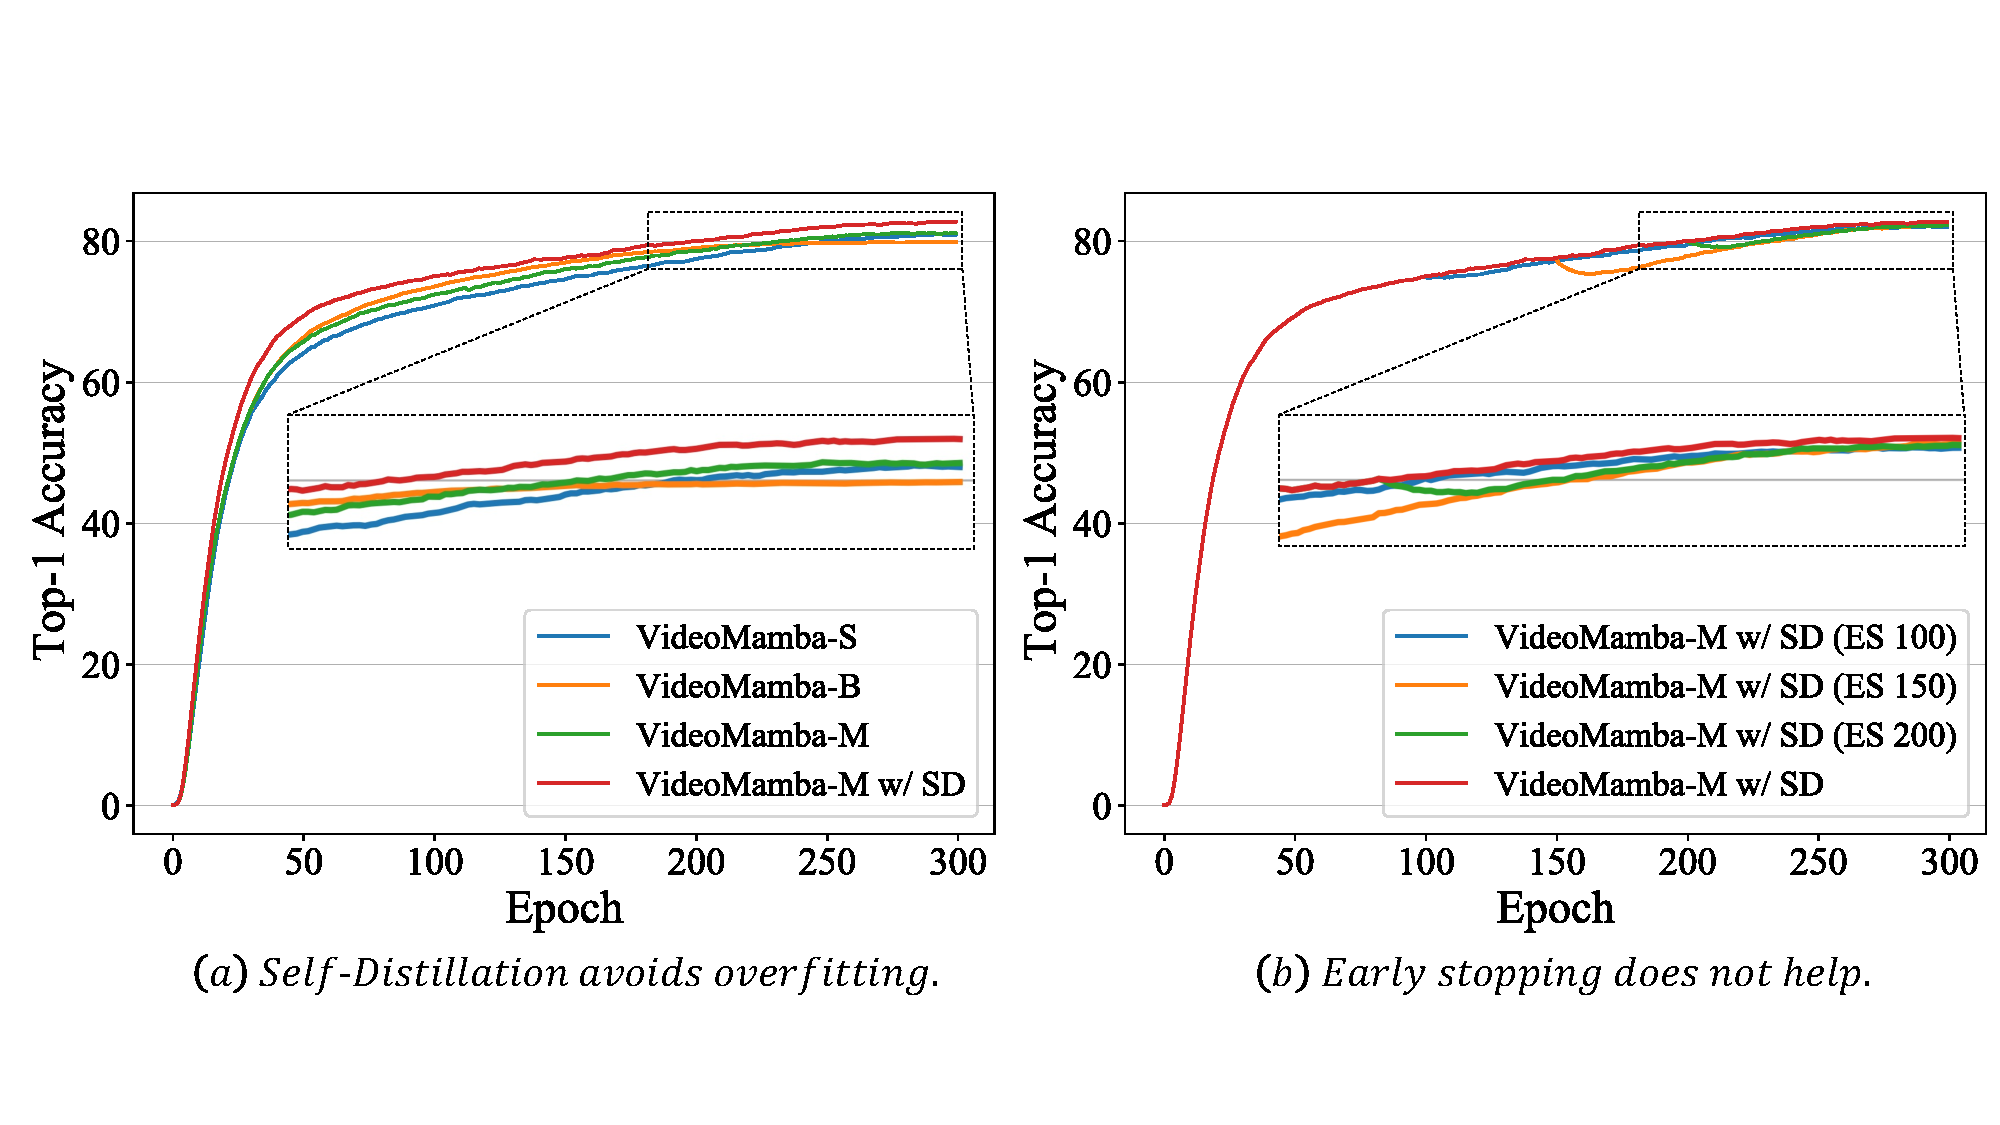
\includegraphics[width=\linewidth]{figs/mamba_imagenet_sd_es_new.pdf} 
\vspace{-0.6cm}
\caption{\textbf{Ablation studies of Self-Distillation and Early Stopping.}
} 
\label{tab:ablation_sd}
\vspace{-0.3cm}
\end{figure}

\noindent\textbf{Dataset and Settings.} 
We first conduct experiments on ImageNet-1K~\cite{imagenet},
which includes 1.28M training images and 50K validation images across 1,000 categories.
For fair comparisons,
we follow most of the training strategies proposed in DeiT~\cite{deit},
but adopt weaker data augmentation for the tiny model variant.
Furthermore,
we adjust the stochastic depth ratio to 0/0.15/0.5 for \ModelName-Ti/S/M.
Our models are trained using the AdamW optimizer paired with a cosine learning rate schedule over 300 epochs. 
The initial 5 epochs serve as a period for linear warm-up. 
Default settings for the learning rate, weight decay, and batch size are 1e-3, 0.05, and 1024, respectively. 
Moreover, 
we use BFloat16 precision during training to enhance stability without relying on EMA.
For the \ModelName-M model, 
we employ a pretrained \ModelName-S model as a ``teacher'' to guide the training process by aligning the final feature maps through L2 loss.
For large resolution ($>$224) fine-tuning,
we use a reduced learning rate (5e-6) and minimal weight decay (1e-8) for 30 epochs.


\vspace{0.05cm}
\noindent\textbf{Effect of Self-Distillation.} 
Fig. \ref{tab:ablation_sd}\red{a} reveals that when trained from scratch,
\ModelName-B tends to overfit more easily and underperforms compared to \ModelName-S, 
whereas \ModelName-M achieves similar performances. 
Fortunately, 
our self-distillation has shown to be effective in achieving the desired optimization with marginal additional computational cost. 
To mitigate teacher's potential overdirection, 
we experimented with early stopping~\cite{early_stopping} in Fig. \ref{tab:ablation_sd}\red{b}, 
although it did not yield beneficial outcomes. 
These findings indicate that self-distillation offers a viable strategy for enhancing the scalability of the Mamba architecture without significant computational overhead.


\begin{table}[tp]
    \vspace{-0.3cm}
    \centering
    \setlength\tabcolsep{6pt}
    \resizebox{0.8\linewidth}{!}{
        \begin{tabular}{l|l|c|r|r|r|c}
        \Xhline{1.0pt}
            \multirow{2}*{\textbf{Arch.}} & \multirow{2}*{\textbf{Model}} & \multirow{2}*{\textit{\textbf{iso.}}} & \textbf{Input} & \textbf{\#Param} & \textbf{FLOPs} & \textbf{IN-1K} \\
            ~ & ~ & ~ & \textbf{Size} & \textbf{(M)} & \textbf{(G)} & \textbf{Top-1}  \\
            \Xhline{0.8pt}
            \multirow{4}{*}{\textbf{\textit{CNN}}} & ConvNeXt-T~\cite{convnext} & \xmark & 224$^2$ & 29 & 4.5 & 82.1 \\
            ~ & ConvNeXt-S~\cite{convnext} & \xmark & 224$^2$ & 50 & 8.7 & 83.1 \\
            ~ & ConvNeXt-B~\cite{convnext} & \xmark & 224$^2$ & 89 & 15.4 & \textbf{83.8} \\
            \hline
            \multirow{4}{*}{\textit{\textbf{Trans.}}}  & SwinT-T~\cite{swin} & \xmark & 224$^2$ & 28 & 4.5 & 81.3 \\
            ~ & Swin-S~\cite{swin} & \xmark & 224$^2$ & 50 & 8.7 & 83.0 \\
            ~ & Swin-B~\cite{swin} & \xmark & 224$^2$ & 88 & 15.4 & 83.5 \\
            \hline
            \multirow{3}{*}{\textit{\textbf{\makecell[l]{CNN+\\SSM}}}}  & VMamba-T~\cite{vmamba} & \xmark & 224$^2$ & 22 & 5.6 & 82.2 \\
            ~ & VMamba-S~\cite{vmamba} & \xmark & 224$^2$ & 44 & 11.2 & 83.5 \\
            ~ & VMamba-B~\cite{vmamba} & \xmark & 224$^2$ & 75 & 18.0 & \underline{83.7} \\
            \Xhline{1.0pt}
            \multirow{2}{*}{\textit{\textbf{CNN}}} & ConvNeXt-S~\cite{convnext} & \cmark & 224$^2$ & 22 & 4.3 & 79.7 \\
            ~ & ConvNeXt-B~\cite{convnext} & \cmark & 224$^2$ & 87 & 16.9 & 82.0 \\
            \hline
            \multirow{4}{*}{\textit{\textbf{Trans.}}}  & DeiT-Ti~\cite{deit} & \cmark & 224$^2$ & 6 & 1.3 & 72.2 \\
            ~ & DeiT-S~\cite{deit} & \cmark & 224$^2$ & 22 & 4.6 & 79.8 \\
            ~ & DeiT-B~\cite{deit} & \cmark & 224$^2$ & 87 & 17.6 & 81.8 \\
            ~ & DeiT-B~\cite{deit} & \cmark & 384$^2$ & 87 & 55.5 & \underline{83.1} \\
            \hline
            \multirow{12}{*}{\textit{\textbf{SSM}}}  & S4ND-ViT-B~\cite{s4nd} & \cmark & 224$^2$ & 89 & - & 80.4 \\
            ~ & Vim-Ti~\cite{vim} & \cmark & 224$^2$ & 7 & 1.1 & 76.1 \\
            ~ & Vim-S~\cite{vim} & \cmark & 224$^2$ & 26 & 4.3 & 80.5 \\
            ~ & \cellcolor{blue!10}{\ModelName-Ti} & \cellcolor{blue!10}{\cmark} & \cellcolor{blue!10}{224$^2$} & \cellcolor{blue!10}{7} & \cellcolor{blue!10}{1.1} & \cellcolor{blue!10}{76.9} \\
            ~ & \cellcolor{blue!10}{\ModelName-Ti} & 
            \cellcolor{blue!10}{\cmark} & \cellcolor{blue!10}{448$^2$} & \cellcolor{blue!10}{7} & \cellcolor{blue!10}{4.3} & \cellcolor{blue!10}{79.3} \\
            ~ & \cellcolor{blue!10}{\ModelName-Ti} & 
            \cellcolor{blue!10}{\cmark} & \cellcolor{blue!10}{576$^2$} & \cellcolor{blue!10}{7} & \cellcolor{blue!10}{7.1} & \cellcolor{blue!10}{79.6} \\
            ~ & \cellcolor{blue!10}{\ModelName-S} & 
            \cellcolor{blue!10}{\cmark} & \cellcolor{blue!10}{224$^2$} & \cellcolor{blue!10}{26} & \cellcolor{blue!10}{4.3} & \cellcolor{blue!10}{81.2} \\
             ~ & \cellcolor{blue!10}{\ModelName-S} & 
            \cellcolor{blue!10}{\cmark} & \cellcolor{blue!10}{448$^2$} & \cellcolor{blue!10}{26} & \cellcolor{blue!10}{16.9} & \cellcolor{blue!10}{83.2} \\
            ~ & \cellcolor{blue!10}{\ModelName-S} & 
            \cellcolor{blue!10}{\cmark} & \cellcolor{blue!10}{576$^2$} & \cellcolor{blue!10}{26} & \cellcolor{blue!10}{28.0} & \cellcolor{blue!10}{83.5} \\
            ~ & \cellcolor{blue!10}{\ModelName-M} & 
            \cellcolor{blue!10}{\cmark} & \cellcolor{blue!10}{224$^2$} & \cellcolor{blue!10}{74} & \cellcolor{blue!10}{12.7} & \cellcolor{blue!10}{82.8} \\
             ~ & \cellcolor{blue!10}{\ModelName-M} & 
            \cellcolor{blue!10}{\cmark} & \cellcolor{blue!10}{448$^2$} & \cellcolor{blue!10}{75} & \cellcolor{blue!10}{50.4} & \cellcolor{blue!10}{83.8} \\
            ~ & \cellcolor{blue!10}{\ModelName-M} & 
            \cellcolor{blue!10}{\cmark} & \cellcolor{blue!10}{576$^2$} & \cellcolor{blue!10}{75} & \cellcolor{blue!10}{83.1} & \cellcolor{blue!10}{\textbf{84.0}} \\
        \Xhline{1.0pt}	
        \end{tabular}
    }
    \caption{\textbf{Comparison with the state-of-the-art on ImageNet.} 
    ``\textit{iso.}'' means isotropic architecture without downsampling layers.
    }
    \label{results_imagenet}
    \vspace{-0.5cm}
\end{table}  


\vspace{0.05cm}
\noindent\textbf{Results.}
Table~\ref{results_imagenet} showcases the results on the ImageNet-1K dataset. 
Notably, 
\ModelName-M outperforms other isotropic architectures by significant margins, achieving a \textbf{+0.8\%} improvement over ConvNeXt-B~\cite{convnext} and a \textbf{+2.0\%} increase compared to DeiT-B~\cite{deit}, 
while utilizing fewer parameters. 
Additionally, \ModelName-M holds its ground against non-isotropic backbones that leverage hierarchical features for enhanced performance. 
Given Mamba's efficiency in processing long sequences, 
we further enhance performance by increasing the resolution, achieving a top-1 accuracy of \textbf{84.0\%} with only 74M parameters. 
This remarkable improvement extends to video tasks, as detailed in Section \ref{sec:short_term}, underscoring \ModelName's effectiveness and scalability.


\begin{table}[t]
    \vspace{-0.3cm}
    \centering
    \setlength\tabcolsep{2pt}
    \resizebox{0.95\linewidth}{!}{
        \begin{tabular}{l|l|c|l|r|r|r|cc}
        \Xhline{1.0pt}
            \multirow{2}*{\textbf{Arch.}} & \multirow{2}*{\textbf{Model}} & \multirow{2}*{\textit{\textbf{iso.}}} & \textbf{Extra} & \textbf{Input} & \textbf{\#Param} & \textbf{FLOPs} & \multicolumn{2}{c}{\textbf{K400}} \\
            ~ & ~ & ~ & \textbf{Data} & \textbf{Size} & \textbf{(M)} & \textbf{(G)} & \textbf{Top-1} & \textbf{Top-5} \\
            \Xhline{0.8pt}
             \multicolumn{9}{l}{\textit{\textbf{\blue{Supervised:}} \gray{Those models with extra data are under supervised training.}}} \\
             \multirow{3}{*}{\textit{\textbf{CNN}}} & SlowFast$_{R101+NL}$~\cite{slowfast} & \xmark &  & 80$\times$224$^2$ & 60 & 234$\times$3$\times$10 & 79.8 & 93.9 \\
             ~ & X3D-M~\cite{x3d} & \xmark &  & 16$\times$224$^2$ & 4 & 6$\times$3$\times$10 & 76.0 & 92.3 \\
             ~ & X3D-XL~\cite{x3d} & \xmark &  & 16$\times$312$^2$ & 20 & 194$\times$3$\times$10 & 80.4 & 94.6 \\
             \hline
             \multirow{3}{*}{\textit{\textbf{Trans.}}} & Swin-T~\cite{video_swin} & \xmark & IN-1K & 32$\times$224$^2$ & 28 & 88$\times$3$\times$4 & 78.8 & 93.6 \\
             ~ & Swin-B~\cite{video_swin} & \xmark & IN-1K & 32$\times$224$^2$ & 88 & 88$\times$3$\times$4 & 80.6 & 94.5 \\
             ~ & Swin-B~\cite{video_swin} & \xmark & IN-21K & 32$\times$224$^2$ & 88 & 282$\times$3$\times$4 & \underline{82.7} & \textbf{95.5} \\
             \hline
             \multirow{5}{*}{\textbf{\textit{\makecell[l]{CNN+\\Trans.}}}} & MViTv1-B~\cite{mvit} & \xmark &  & 32$\times$224$^2$ & 37 & 70$\times$1$\times$5 & 80.2 & 94.4 \\
             ~ & MViTv2-S~\cite{mvitv2} & \xmark &  & 16$\times$224$^2$ & 35 & 64$\times$1$\times$5 & 81.0 & 94.6 \\
             ~ & UniFormer-S~\cite{uniformer} & \xmark & IN-1K & 16$\times$224$^2$ & 21 & 42$\times$1$\times$4 & 80.8 & 94.7 \\
             ~ & UniFormer-B~\cite{uniformer} & \xmark & IN-1K & 16$\times$224$^2$ & 50 & 97$\times$1$\times$4 & 82.0 & 95.1 \\
             ~ & UniFormer-B~\cite{uniformer} & \xmark & IN-1K & 32$\times$224$^2$ & 50 & 259$\times$3$\times$4 & \textbf{83.0} & \underline{95.4} \\
             \Xhline{0.8pt}
             \multirow{4}{*}{\textit{\textbf{Trans.}}} & STAM~\cite{stam} & \cmark & IN-21K & 64$\times$224$^2$ & 121 & 1040$\times$1$\times$1 & 79.2 & - \\
             ~ & TimeSformer-L~\cite{timesformer} & \cmark & IN-21K & 96$\times$224$^2$ & 121 & 2380$\times$3$\times$1 & 80.7 & 94.7 \\
             ~ & ViViT-L~\cite{vivit} & \cmark & IN-21K & 16$\times$224$^2$ & 311 & 3992$\times$3$\times$4 & \underline{81.3} & 94.7 \\
             ~ & Mformer-HR~\cite{motionformer} & \cmark & IN-21K & 16$\times$336$^2$ & 311 & 959$\times$3$\times$10 & 81.1 & \underline{95.2} \\
             \hline
             \multirow{9}{*}{\textit{\textbf{SSM}}} & \cellcolor{blue!10}{\ModelName-Ti} & \cellcolor{blue!10}{\cmark} & \cellcolor{blue!10}{IN-1K} & \cellcolor{blue!10}{16$\times$224$^2$} & \cellcolor{blue!10}{7} & \cellcolor{blue!10}{17$\times$3$\times$4} & \cellcolor{blue!10}{78.1} & \cellcolor{blue!10}{93.5} \\
             ~ & \cellcolor{blue!10}{\ModelName-Ti} & \cellcolor{blue!10}{\cmark} & \cellcolor{blue!10}{IN-1K} & \cellcolor{blue!10}{32$\times$224$^2$} & \cellcolor{blue!10}{7} & \cellcolor{blue!10}{34$\times$3$\times$4} & \cellcolor{blue!10}{78.8} & \cellcolor{blue!10}{93.9} \\
             ~ & \cellcolor{blue!10}{\ModelName-Ti} & \cellcolor{blue!10}{\cmark} & \cellcolor{blue!10}{IN-1K} & \cellcolor{blue!10}{64$\times$384$^2$} & \cellcolor{blue!10}{7} & \cellcolor{blue!10}{202$\times$3$\times$4} & \cellcolor{blue!10}{80.3} & \cellcolor{blue!10}{94.8} \\


             ~ & \cellcolor{blue!10}{\ModelName-S} & \cellcolor{blue!10}{\cmark} & \cellcolor{blue!10}{IN-1K} & \cellcolor{blue!10}{16$\times$224$^2$} & \cellcolor{blue!10}{26} & \cellcolor{blue!10}{68$\times$3$\times$4} & \cellcolor{blue!10}{80.8} & \cellcolor{blue!10}{94.8} \\
             ~ & \cellcolor{blue!10}{\ModelName-S} & \cellcolor{blue!10}{\cmark} & \cellcolor{blue!10}{IN-1K} & \cellcolor{blue!10}{32$\times$224$^2$} & \cellcolor{blue!10}{26} & \cellcolor{blue!10}{135$\times$3$\times$4} & \cellcolor{blue!10}{81.5} & \cellcolor{blue!10}{95.2} \\
             ~ & \cellcolor{blue!10}{\ModelName-S} & \cellcolor{blue!10}{\cmark} & \cellcolor{blue!10}{IN-1K} & \cellcolor{blue!10}{64$\times$384$^2$} & \cellcolor{blue!10}{26} & \cellcolor{blue!10}{395$\times$3$\times$4} & \cellcolor{blue!10}{82.7} & \cellcolor{blue!10}{95.6} \\

             ~ & \cellcolor{blue!10}{\ModelName-M} & \cellcolor{blue!10}{\cmark} & \cellcolor{blue!10}{IN-1K} & \cellcolor{blue!10}{16$\times$224$^2$} & \cellcolor{blue!10}{74} & \cellcolor{blue!10}{202$\times$3$\times$4} & \cellcolor{blue!10}{81.9} & \cellcolor{blue!10}{95.4} \\
             ~ & \cellcolor{blue!10}{\ModelName-M} & \cellcolor{blue!10}{\cmark} & \cellcolor{blue!10}{IN-1K} & \cellcolor{blue!10}{32$\times$224$^2$} & \cellcolor{blue!10}{74} & \cellcolor{blue!10}{403$\times$3$\times$4} & \cellcolor{blue!10}{82.4} & \cellcolor{blue!10}{95.7} \\
             ~ & \cellcolor{blue!10}{\ModelName-M} & \cellcolor{blue!10}{\cmark} & \cellcolor{blue!10}{IN-1K} & \cellcolor{blue!10}{64$\times$384$^2$} & \cellcolor{blue!10}{74} & \cellcolor{blue!10}{2368$\times$3$\times$4} & \cellcolor{blue!10}{\textbf{83.3}} & \cellcolor{blue!10}{\textbf{96.1}} \\
             
             \Xhline{1.0pt}
             \multicolumn{9}{l}{\textit{\textbf{\blue{Self-supervised:}} \gray{For UMT, the CLIP-400M is used in pretrained teacher.}}} \\
             \multirow{5}{*}{\textit{\textbf{Trans.}}} & BEVT-B$_{800e}$~\cite{bevt} & \xmark & IN-1K & 32$\times$224$^2$ & 88 & 282$\times$3$\times$4 & 81.1 & - \\
             \cline{2-9}
             ~ & ST-MAE-B$_{1600e}$~\cite{st_mae} & \cmark &  & 16$\times$224$^2$ & 87 & 180$\times$3$\times$7 & 81.3 & 94.9 \\
             ~ & VideoMAE-S$_{2400e}$~\cite{videomae} & \cmark &  & 16$\times$224$^2$ & 22 & 57$\times$3$\times$5 & 79.0 & 93.8 \\
             ~ & VideoMAE-B$_{1600e}$~\cite{videomae} & \cmark &  & 16$\times$224$^2$ & 87 & 180$\times$3$\times$5 & 81.5 & 95.1 \\
             ~ & UMT-B$_{800e}$~\cite{umt} & \cmark & \gray{CLIP-400M} & 8$\times$224$^2$ & 87 & 180$\times$3$\times$5 & \textbf{85.7} & \textbf{97.0} \\

             \hline
             \multirow{4}{*}{\textit{\textbf{SSM}}} & \cellcolor{blue!10}{\ModelName-M$_{800e}$} & \cellcolor{blue!10}{\cmark} & \cellcolor{blue!10}{\gray{CLIP-400M}} & \cellcolor{blue!10}{8$\times$224$^2$} & \cellcolor{blue!10}{74} & \cellcolor{blue!10}{101$\times$3$\times$4} & \cellcolor{blue!10}{82.0} & \cellcolor{blue!10}{95.4} \\
             ~ & \cellcolor{blue!10}{\ModelName-M$_{800e}$} & \cellcolor{blue!10}{\cmark} & \cellcolor{blue!10}{\gray{CLIP-400M}} & \cellcolor{blue!10}{16$\times$224$^2$} & \cellcolor{blue!10}{74} & \cellcolor{blue!10}{202$\times$3$\times$4} & \cellcolor{blue!10}{83.4} & \cellcolor{blue!10}{95.9} \\
             ~ & \cellcolor{blue!10}{\ModelName-M$_{800e}$} & \cellcolor{blue!10}{\cmark} & \cellcolor{blue!10}{\gray{CLIP-400M}} & \cellcolor{blue!10}{32$\times$224$^2$} & \cellcolor{blue!10}{74} & \cellcolor{blue!10}{403$\times$3$\times$4} &\cellcolor{blue!10}{83.9} & \cellcolor{blue!10}{96.2} \\
             ~ & \cellcolor{blue!10}{\ModelName-M$_{800e}$} & \cellcolor{blue!10}{\cmark} & \cellcolor{blue!10}{\gray{CLIP-400M}} & \cellcolor{blue!10}{64$\times$384$^2$} & \cellcolor{blue!10}{74} & \cellcolor{blue!10}{2368$\times$3$\times$4} &\cellcolor{blue!10}{\underline{85.0}} & \cellcolor{blue!10}{\underline{96.9}} \\
        \Xhline{1.0pt}	
        \end{tabular}
    }
    \caption{\textbf{Comparison with the state-of-the-art on scene-related Kinetics-400.} 
    ``\textit{iso.}'' means isotropic architecture without downsampling layers.
    Masked modeling~\cite{umt} also works for Mamba,
    but the inconsistent architecture leads to inferior alignment.
    }
    \label{results_k400}
    \vspace{-0.6cm}
\end{table}  

\begin{table}[t]
    \vspace{-0.3cm}
    \centering
    \setlength\tabcolsep{2pt}
    \resizebox{0.96\linewidth}{!}{
        \begin{tabular}{l|l|c|l|r|r|r|cc}
        \Xhline{1.0pt}
            \multirow{2}*{\textbf{Arch.}} & \multirow{2}*{\textbf{Model}} & \multirow{2}*{\textit{\textbf{iso.}}} & \textbf{Extra} & \textbf{Input} & \textbf{\#Param} & \textbf{FLOPs} & \multicolumn{2}{c}{\textbf{SSV2}} \\
            ~ & ~ & ~ & \textbf{Data} & \textbf{Size} & \textbf{(M)} & \textbf{(G)} & \textbf{Top-1} & \textbf{Top-5} \\
            \Xhline{0.8pt}
             \multicolumn{9}{l}{\textit{\textbf{\blue{Supervised:}} \gray{Those models with extra data are under supervised training.}}} \\
             \multirow{3}{*}{\textit{\textbf{CNN}}} & SlowFast$_{R101}$~\cite{slowfast} & \xmark & K400 & 32$\times$224$^2$ & 53 & 106$\times$3$\times$1 & 63.1 & 87.6 \\
             ~ & CT-Net$_{R50}$~\cite{ct_net} & \xmark & IN-1K & 16$\times$224$^2$ & 21 & 75$\times$1$\times$1 & 64.5 & 89.3 \\
             ~ & TDN$_{R50}$~\cite{tdn} & \xmark & IN-1K & 16$\times$224$^2$ & 26 & 75$\times$1$\times$1 & 65.3 & 91.6 \\
             \hline
             \multirow{1}{*}{\textit{\textbf{Trans.}}} & Swin-B~\cite{video_swin} & \xmark & K400 & 32$\times$224$^2$ & 89 & 88$\times$3$\times$1 & 69.6 & 92.7 \\
             \hline
             \multirow{6}{*}{\textbf{\textit{\makecell[l]{CNN+\\Trans.}}}} & MViTv1-B~\cite{mvit} & \xmark & K400 & 16$\times$224$^2$ & 37 & 71$\times$3$\times$1 & 64.7 & 89.2 \\
             ~ & MViTv1-B~\cite{mvit} & \xmark & K400 & 32$\times$224$^2$ & 37 & 170$\times$3$\times$1 & 67.1 & 90.8 \\
             ~ & MViTv2-S~\cite{mvitv2} & \xmark & K400 & 16$\times$224$^2$ & 35 & 65$\times$3$\times$1 & 68.2 & 91.4 \\
             ~ & MViTv2-B~\cite{mvitv2} & \xmark & K400 & 32$\times$224$^2$ & 51 & 225$\times$3$\times$1 & \textbf{70.5} & \underline{92.7} \\
             ~ & UniFormer-S~\cite{uniformer} & \xmark & \scriptsize{IN-1K+K400} & 16$\times$224$^2$ & 21 & 42$\times$3$\times$1 & 67.7 & 91.4 \\
             ~ & UniFormer-B~\cite{uniformer} & \xmark & \scriptsize{IN-1K+K400} & 16$\times$224$^2$ & 50 & 97$\times$3$\times$1 & \underline{70.4} & \textbf{92.8} \\
             \Xhline{0.8pt}
             \multirow{3}{*}{\textit{\textbf{Trans.}}} & TimeSformer-HR~\cite{timesformer} & \cmark & IN-21K & 16$\times$224$^2$ & 121 & 1703$\times$3$\times$1 & 62.5 & - \\
             ~ & ViViT-L~\cite{vivit} & \cmark & \scriptsize{IN-21K+K400} & 16$\times$224$^2$ & 311 & 3992$\times$3$\times$4 & 65.4 & 89.8 \\
             ~ & Mformer-HR~\cite{motionformer} & \cmark & \scriptsize{IN-21K+K400} & 16$\times$336$^2$ & 311 & 1185$\times$3$\times$1 & \underline{68.1} & \underline{91.2} \\
             \hline
             \multirow{9}{*}{\textit{\textbf{SSM}}} & \cellcolor{blue!10}{\ModelName-Ti} & \cellcolor{blue!10}{\cmark} & \cellcolor{blue!10}{IN-1K} & \cellcolor{blue!10}{8$\times$224$^2$} & \cellcolor{blue!10}{7} & \cellcolor{blue!10}{9$\times$3$\times$2} & \cellcolor{blue!10}{65.1} & \cellcolor{blue!10}{89.1} \\
             ~ & \cellcolor{blue!10}{\ModelName-Ti} & \cellcolor{blue!10}{\cmark} & \cellcolor{blue!10}{IN-1K} & \cellcolor{blue!10}{16$\times$224$^2$} & \cellcolor{blue!10}{7} & \cellcolor{blue!10}{17$\times$3$\times$2} & \cellcolor{blue!10}{66.0} & \cellcolor{blue!10}{89.6} \\
             ~ & \cellcolor{blue!10}{\ModelName-Ti} & \cellcolor{blue!10}{\cmark} & \cellcolor{blue!10}{IN-1K} & \cellcolor{blue!10}{16$\times$288$^2$} & \cellcolor{blue!10}{7} & \cellcolor{blue!10}{28$\times$3$\times$2} & \cellcolor{blue!10}{66.2} & \cellcolor{blue!10}{90.0} \\


             ~ & \cellcolor{blue!10}{\ModelName-S} & \cellcolor{blue!10}{\cmark} & \cellcolor{blue!10}{IN-1K} & \cellcolor{blue!10}{8$\times$224$^2$} & \cellcolor{blue!10}{26} & \cellcolor{blue!10}{34$\times$3$\times$2} & \cellcolor{blue!10}{66.6} & \cellcolor{blue!10}{90.4} \\
             ~ & \cellcolor{blue!10}{\ModelName-S} &\cellcolor{blue!10}{\cmark} & \cellcolor{blue!10}{IN-1K} & \cellcolor{blue!10}{16$\times$224$^2$} & \cellcolor{blue!10}{26} & \cellcolor{blue!10}{68$\times$3$\times$2} & \cellcolor{blue!10}{67.6} & \cellcolor{blue!10}{90.9} \\
             ~ & \cellcolor{blue!10}{\ModelName-S} &\cellcolor{blue!10}{\cmark} & \cellcolor{blue!10}{IN-1K} & \cellcolor{blue!10}{16$\times$288$^2$} & \cellcolor{blue!10}{26} & \cellcolor{blue!10}{112$\times$3$\times$2} & \cellcolor{blue!10}{68.1} & \cellcolor{blue!10}{91.2} \\

             ~ & \cellcolor{blue!10}{\ModelName-M} & \cellcolor{blue!10}{\cmark} & \cellcolor{blue!10}{IN-1K} & \cellcolor{blue!10}{8$\times$224$^2$} & \cellcolor{blue!10}{74} & \cellcolor{blue!10}{101$\times$3$\times$4} & \cellcolor{blue!10}{67.3} & \cellcolor{blue!10}{91.0} \\
             ~ & \cellcolor{blue!10}{\ModelName-M} & \cellcolor{blue!10}{\cmark} & \cellcolor{blue!10}{IN-1K} & \cellcolor{blue!10}{16$\times$224$^2$} & \cellcolor{blue!10}{74} & \cellcolor{blue!10}{202$\times$3$\times$4} & \cellcolor{blue!10}{68.3} & \cellcolor{blue!10}{91.4} \\
             ~ & \cellcolor{blue!10}{\ModelName-M} & \cellcolor{blue!10}{\cmark} & \cellcolor{blue!10}{IN-1K} & \cellcolor{blue!10}{16$\times$288$^2$} & \cellcolor{blue!10}{74} & \cellcolor{blue!10}{333$\times$3$\times$4} & \cellcolor{blue!10}{\textbf{68.4}} & \cellcolor{blue!10}{\textbf{91.6}} \\
             
             \Xhline{1.0pt}
             \multicolumn{9}{l}{\textit{\textbf{\blue{Self-supervised:}} \gray{For UMT, the CLIP-400M is used in pretrained teacher.}}} \\
             \multirow{4}{*}{\textit{\textbf{Trans.}}} & BEVT-B$_{800e}$~\cite{bevt} & \xmark & \scriptsize{IN-1K+K400} & 32$\times$224$^2$ & 88 & 321$\times$3$\times$1 & 70.6 & - \\
             \cline{2-9}
             ~ & VideoMAE-S$_{2400e}$~\cite{videomae} & \cmark &  & 16$\times$224$^2$ & 22 & 57$\times$3$\times$2 & 66.8 & 90.3 \\
             ~ & VideoMAE-B$_{2400e}$~\cite{videomae} & \cmark &  & 16$\times$224$^2$ & 87 & 180$\times$3$\times$2 & \underline{70.8} & 92.4 \\
             ~ & UMT-B$_{800e}$~\cite{umt} & \cmark & \gray{CLIP-400M} & 8$\times$224$^2$ & 87 & 180$\times$3$\times$2 & \underline{70.8} & \underline{92.6} \\

             \hline
             \multirow{3}{*}{\textit{\textbf{SSM}}} & \cellcolor{blue!10}{\ModelName-M$_{800e}$} & \cellcolor{blue!10}{\cmark} & \cellcolor{blue!10}{\gray{CLIP-400M}} & \cellcolor{blue!10}{8$\times$224$^2$} & \cellcolor{blue!10}{74} & \cellcolor{blue!10}{101$\times$3$\times$2} & \cellcolor{blue!10}{70.2} & \cellcolor{blue!10}{92.6} \\
             ~ & \cellcolor{blue!10}{\ModelName-M$_{800e}$} & \cellcolor{blue!10}{\cmark} & \cellcolor{blue!10}{\gray{CLIP-400M}} & \cellcolor{blue!10}{16$\times$224$^2$} & \cellcolor{blue!10}{74} & \cellcolor{blue!10}{202$\times$3$\times$2} & \cellcolor{blue!10}{71.0} & \cellcolor{blue!10}{92.7} \\
             ~ & \cellcolor{blue!10}{\ModelName-M$_{800e}$} & \cellcolor{blue!10}{\cmark} & \cellcolor{blue!10}{\gray{CLIP-400M}} & \cellcolor{blue!10}{16$\times$288$^2$} & \cellcolor{blue!10}{74} & \cellcolor{blue!10}{333$\times$3$\times$2} & \cellcolor{blue!10}{\textbf{71.4}} & \cellcolor{blue!10}{\textbf{92.9}} \\
        \Xhline{1.0pt}	
        \end{tabular}
    }
    \caption{\textbf{Comparison with the state-of-the-art on temporal-related SthSth V2.} 
    ``\textit{iso.}'' means isotropic architecture without downsampling layers.
    Masked modeling~\cite{umt} also works for Mamba, 
    and it performs better than VideoMAE.
    }
    \label{results_ssv2}
    \vspace{-0.6cm}
\end{table}  


\subsection{Short-term Video Understanding}
\label{sec:short_term}


\noindent\textbf{Datasets and Settings.} 
We evaluate our \ModelName\  on the popular scene-related Kinetics-400~\cite{k400} and temporal-related Something-Something V2~\cite{sth},
the average video lengths of which are 10s and 4s.
For supervised pretraining,
we fine-tune those models pretrained on ImageNet-1K with the same training strategy as VideoMAE~\cite{videomae}.
Specifically,
for \ModelName-M,
the warmup epoch, total epoch, stochastic depth rate, weight decay are set to 5, 50, 0.8, 0.05 for K400,
and 5, 30, 0.8, 0.05 for SthSth.
For the smaller models,
all the hyper-parameters are the same unless we decrease the stochastic depth rate and increase the training epochs.
Moreover, 
we linearly scale the base learning rates according to the batch size,
which are $2e^{-4}\cdot\frac{batchsize}{256}$ for K400 and $4e^{-4}\cdot\frac{batchsize}{256}$ for SthSth.
As for self-supervised pretraining,
we adopt the training recipe as in UMT~\cite{umt},
employing CLIP-ViT-B~\cite{clip} to distill \ModelName-M over 800 epochs. 
During fine-tuning,
we use similar hyperparameters as mentioned but opt for a small stochastic depth rate and learning rate for both datasets.


\vspace{0.05cm}
\noindent\textbf{Results.}
Table \ref{results_k400} and \ref{results_ssv2} list the results on short-term video datasets.
\textbf{(a) \textit{Supervised}:}
Compared with the purely attention-based methods~\cite{timesformer,vivit},
our SSM-based \ModelName-M secures a notable advantage, 
outperforming ViViT-L~\cite{vivit} by \textbf{+2.0\%} and \textbf{+3.0\%} on the scene-related K400 and the temporally-related SthSthV2 datasets, respectively. 
This improvement comes with significantly reduced computational demands and less pretraining data.
Furthermore, 
\ModelName-M delivers results that are on par with the SOTA UniFormer~\cite{uniformer}, 
which skillfully integrates convolution with attention in a non-isotropic structure.
\textbf{(b) \textit{Self-supervised}:}
The performance of \ModelName\  under masked pretraining surpasses that of the VideoMAE~\cite{videomae}, 
known for its proficiency in fine-grained action. This achievement underscores the potential of our purely SSM-based model in efficiently and effectively understanding short-term videos, highlighting its suitability for both supervised and self-supervised learning paradigms.


\vspace{0.05cm}
\noindent\textbf{Ablation Studies.} 
Through comprehensive ablation studies detailed in Fig. \ref{tab:ablation_scan_frame_resolution} and Table \ref{ablation_mask}, 
we explore various aspects of our model.
\textbf{(a) \textit{Scan Type}:}
Among all the methods,
the spatial-first approach emerges as the most effective, 
in contrast, 
the temporal-first strategy is the worst. 
The superiority of the spatial-first method is attributed to its ability to seamlessly leverage 2D pretrained knowledge by scanning frame by frame.
\textbf{(b) \textit{Frame and Resolution}:}
Contrary to findings from ImageNet (see Table \ref{results_imagenet}), 
higher resolution does not uniformly lead to better performance. 
Increasing the number of frames consistently enhances results on the K400 dataset. 
However, 
this is not the case with SthSthV2, 
possibly due to the brief duration of its videos, which may not accommodate longer inputs effectively.
\textbf{(c) \textit{Masked Pretraining}:}
Our findings reveal that row masking, 
being particularly compatible with 1D convolution, outperforms commonly used random and tube masking. 
Clip-row masking excels owing to its higher degree of randomness. 
Moreover, 
attention masking stands out as the most efficient by favoring the preservation of adjacent meaningful content. 
Aligning solely the model's final output proves most effective, 
likely due to architectural differences. 
Lastly, an optimal masking ratio (80\%) combined with stronger regularization significantly benefits \ModelName\  during masked pretraining.


\begin{figure}[t]
\vspace{-0.3cm}
\centering
\begin{minipage}{0.3\textwidth}
\centering
    \vspace{0pt}
    \centering
    \setlength\tabcolsep{1pt}
    \resizebox{\textwidth}{!}{
        \begin{tabular}{l|c}
            \textbf{Type} & \textbf{SSV2} \\
            \Xhline{1.0pt}
            \rowcolor{gray!20}
            SF-Bidirectional & \textbf{65.1} \\
            TF-Bidirectional & 62.4 \\
            ST-Bidirectional v1 & 63.9 \\
            ST-Bidirectional v2 & 64.2 \\
            Half-SF + Half-TF & 64.0 \\
            Half-TF + Half-SF & 64.1 \\
            Alternative SF\&TF & \textbf{65.1} \\
        \end{tabular}
    }
    % \vspace{-0.2cm}
    \subcaption{
        \textbf{Scan Type.}
        Spatial-First scan is simple yet effective.
    }
    \label{tab:ablation_scan}
\end{minipage}
\begin{minipage}{0.69\textwidth}

\begin{minipage}{0.49\textwidth}
    \vspace{0pt}
    \centering
    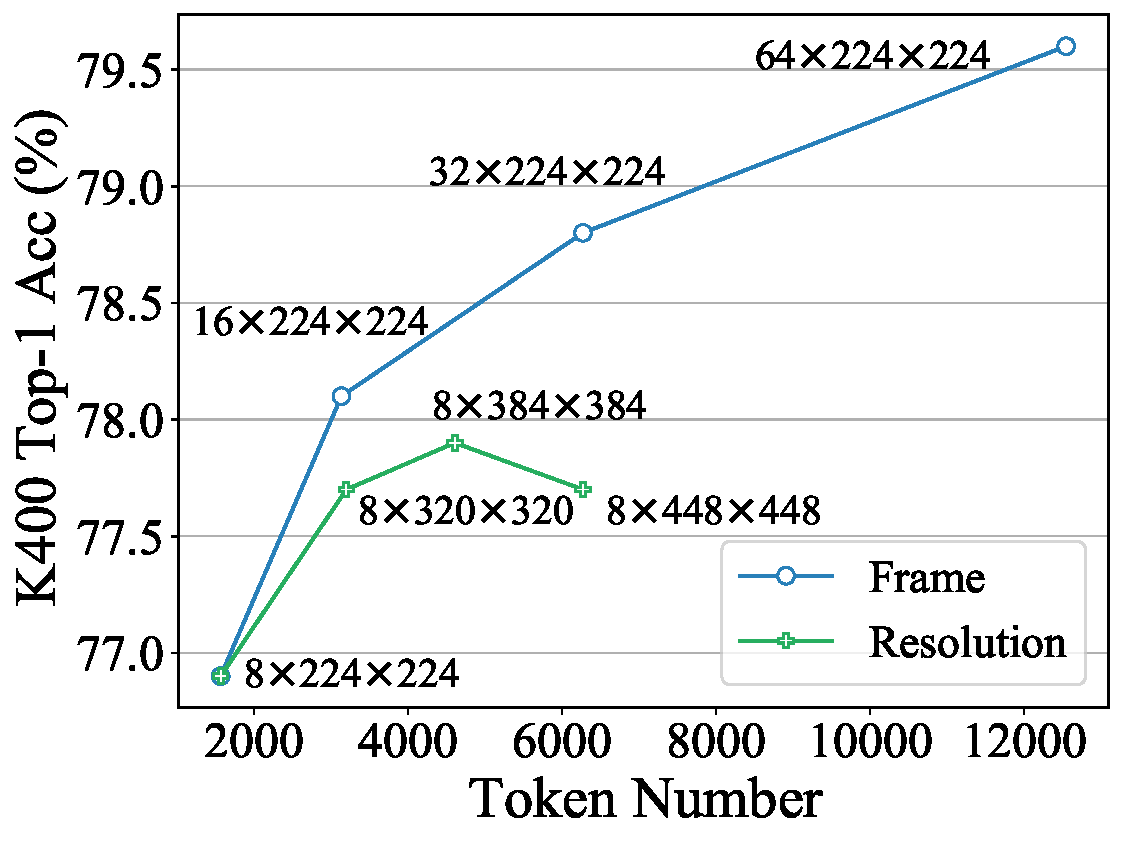
\includegraphics[width=\linewidth]{figs/mamba_k400.pdf}
    % \subcaption{\textbf{K400.}}
\end{minipage}
% \hfill
\begin{minipage}{0.49\textwidth}
    \vspace{0pt}
    \centering
    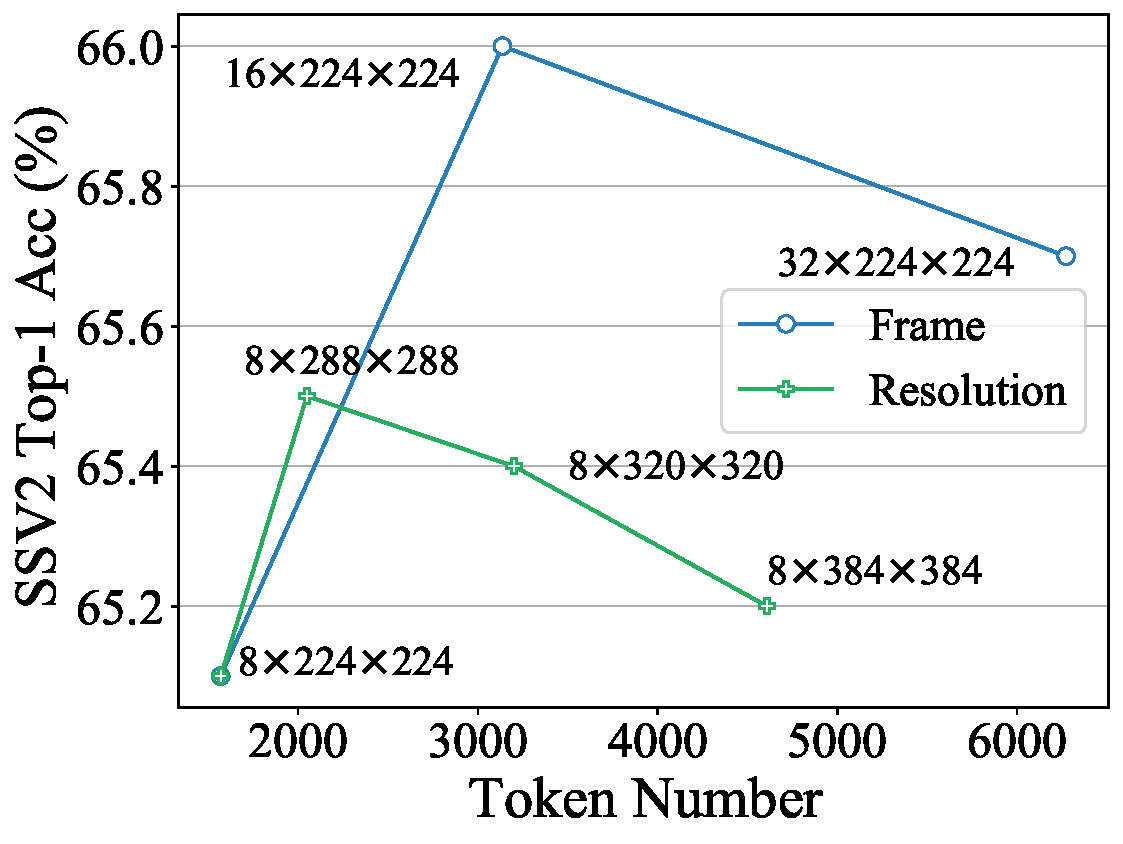
\includegraphics[width=\linewidth]{figs/mamba_ssv2.pdf} 
    % \subcaption{\textbf{SSV2.}}
\end{minipage}
\subcaption{\textbf{Frame \& Resolution for K400 and SSV2.}}
\end{minipage}
\vspace{-0.3cm}
\caption{\textbf{Ablation studies of scan type, frame and resolution.}
All the models are fine-tuned from \ModelName-Ti pretrained on ImageNet.
} 
\label{tab:ablation_scan_frame_resolution}
\vspace{-0.3cm}
\end{figure}

\begin{table}[t]
    \begin{minipage}[t]{0.27\linewidth}
        \vspace{0pt}
        \centering
        \setlength\tabcolsep{8.0pt}
        \resizebox{\textwidth}{!}{
            \begin{tabular}{l|c}
                \textbf{Type} & \textbf{SSV2} \\
                \Xhline{1.0pt}
                Random & 67.4 \\
                Tube & 66.3 \\
                Clip-Row & 68.2 \\
                Frame-Row & 67.8 \\
                \rowcolor{gray!20}
                Attention & \textbf{68.5} \\
            \end{tabular}
        }
        % \vspace{-0.2cm}
        \subcaption{
            \textbf{Mask Type.}
        }
        \label{ablation_mask_type}
    \end{minipage}
    \hspace{0.3mm}
    \ 
    \begin{minipage}[t]{0.25\linewidth}
        \vspace{0pt}
        \centering
        \setlength\tabcolsep{6.5pt}
        \resizebox{\textwidth}{!}{
            \begin{tabular}{l|c}
                \textbf{Layer} & \textbf{SSV2} \\
                \Xhline{1.0pt}
                \rowcolor{gray!20}
                Last 1 & \textbf{68.5} \\
                Last 2 & 68.4 \\
                Last 6 & 68.2 \\
                Last 6$\times$2 & 67.7 \\
            \end{tabular}
        }
        % \vspace{-0.2cm}
        \subcaption{
            \textbf{Alignment Layer.}
        }
        \label{ablation_mask_layer}
    \end{minipage}
    \hspace{0.3mm}
    \ 
    \begin{minipage}[t]{0.22\linewidth}
        \vspace{0pt}
        \centering
        \setlength\tabcolsep{6.5pt}
        \resizebox{\textwidth}{!}{
            \begin{tabular}{l|c}
                \textbf{Ratio} & \textbf{SSV2} \\
                \Xhline{1.0pt}
                50\% & 68.1 \\
                65\% & 68.4 \\
                \rowcolor{gray!20}
                80\% & \textbf{68.5} \\
                90\% & 68.2 \\
            \end{tabular}
        }
        % \vspace{-0.2cm}
        \subcaption{
            \textbf{Mask Ratio.}
        }
        \label{ablation_mask_ratio}
    \end{minipage}
    \hspace{0.3mm}
    \ 
    \begin{minipage}[t]{0.18\linewidth}
        \vspace{0pt}
        \centering
        \setlength\tabcolsep{5.2pt}
        \resizebox{\textwidth}{!}{
            \begin{tabular}{l|c}
                \textbf{DP} & \textbf{SSV2} \\
                \Xhline{1.0pt}
                0.1 & 68.0 \\
                0.2 & 68.2 \\
                0.3 & 68.4 \\
                \rowcolor{gray!20}
                0.4 & \textbf{68.5} \\
            \end{tabular}
        }
        % \vspace{-0.2cm}
        \subcaption{
            \textbf{Droppath.}
        }
        \label{ablation_mask_droppath}
    \end{minipage}
    \vspace{-0.3cm}
    \caption{
        \textbf{Ablation studies of masked pretraining.}
        We adopt CLIP-ViT-B~\cite{clip} as a teacher to distill \ModelName-M for 200 epochs.
    }
    \label{ablation_mask}
    \vspace{-0.5cm}
\end{table}




\subsection{Long-term Video Understanding}



\begin{table}[t]
    \vspace{-0.3cm}
    \centering
    \setlength\tabcolsep{2pt}
    \resizebox{0.95\linewidth}{!}{
        \begin{tabular}{l|c|l|l|l|cc}
        \Xhline{1.0pt}
            \multirow{2}*{\textbf{Method}} & \multirow{2}*{\textit{\textbf{e2e}}} & \multirow{2}*{\textbf{Backbone}} & \multirow{2}*{\textbf{Neck Type}} & \textbf{Pretraining}  & \textbf{BF} & \textbf{COIN} \\
            ~ & ~ & ~ & ~ & \textbf{Dataset} & \textbf{Top-1} & \textbf{Top-1} \\
            \Xhline{0.8pt}
             Timeception~\cite{timeception} & \xmark & 3D-ResNet & Conv. & IN-1K+K400 & 71.3 & - \\
             VideoGraph~\cite{videograph} & \xmark & I3D & Conv.+Atten. & IN-1K+K400 & 69.5 & - \\
             GHRM~\cite{ghrm} & \xmark & I3D & Graph Conv.. & IN-1K+K400 & 75.5 & - \\
             % TimeSformer~\cite{distant} & \xmark & TimeSformer & Attention & K400 & 81.1 & 83.5 \\
             % Distant Supervision~\cite{distant} & \xmark & TimeSformer & Atten. & IN-21K+HTM & 88.7 & 88.9 \\
             Distant Supervision~\cite{distant} & \xmark & TimeSformer & Atten. w/ KB & IN-21K+HTM & \textbf{89.9} & \textbf{90.0} \\
             ViS4mer~\cite{vis4mer} & \xmark & Swin-B & SSM & IN-21K+K600 & \underline{88.2} & \underline{88.4} \\
             \Xhline{0.8pt}
             Turbo$_{f32}$~\cite{turbo} & \cmark & VideoMAE-B &  & K400 & 86.8 & 82.3 \\
             Turbo$_{f32}$~\cite{turbo} & \cmark & VideoMAE-B &  & K400+HTM-AA & \underline{91.3} & \underline{87.5} \\
             \rowcolor{blue!10}
             \ModelName$_{f32}$ & \cmark & \ModelName-Ti &  & K400 & 94.3 & 86.2 \\
             \rowcolor{blue!10}
             \ModelName$_{f64}$ & \cmark & \ModelName-Ti &  & K400 & 94.3 & 87.0 \\
             \rowcolor{blue!10}
             \ModelName$_{f32}$ & \cmark & \ModelName-S &  & K400 & 95.3 & 88.4 \\
             \rowcolor{blue!10}
             \ModelName$_{f64}$ & \cmark & \ModelName-S &  & K400 & 97.4 & 88.7 \\
             \rowcolor{blue!10}
             \ModelName$_{f32}$ & \cmark & \ModelName-M &  & K400 & 94.8 & 88.3 \\
             \rowcolor{blue!10}
             \ModelName$_{f64}$ & \cmark & \ModelName-M &  & K400 & 95.8 & 89.5 \\
             \rowcolor{blue!10}
             \ModelName$_{f32}$ & \cmark & \ModelName-M\myred{$\dag$} &  & K400 & \textbf{97.9} & 89.6 \\
             \rowcolor{blue!10}
             \ModelName$_{f64}$ & \cmark & \ModelName-M\myred{$\dag$} &  & K400 & 96.9 & \textbf{90.4} \\
        \Xhline{1.0pt}	
        \end{tabular}
    }
    \caption{\textbf{Comparison with the state-of-the-art on Breakfast and COIN.} 
    ``\textit{e2e}'' means end-to-end methods without exhausting feature extraction.
    ``\myred{$\dag$}'' marks the backbone with masked pretraining.
    }
    \label{results_breakfast_coin}
    \vspace{-0.6cm}
\end{table}  

\begin{table}[t]
    \centering
    \setlength\tabcolsep{2pt}
    \resizebox{0.98\linewidth}{!}{
        \begin{tabular}{l|c|l|ccc|cccc|cc}
        \Xhline{1.0pt}
            \multirow{2}*{\textbf{Method}} & \multirow{2}*{\textit{\textbf{e2e}}} & \multirow{2}*{\textit{\textbf{Backbone}}} & \multicolumn{3}{c|}{\textbf{Content($\uparrow$)}} & \multicolumn{4}{c|}{\textbf{Metadata($\uparrow$)}} & \multicolumn{2}{c}{\textbf{User($\downarrow$)}} \\
            ~ & ~ & ~ & \textbf{Rel.} & \textbf{Speak} & \textbf{Scene} & \textbf{Dir.} & \textbf{Genre} & \textbf{Wtr.} & \textbf{Year} & \textbf{Like} & \textbf{View} \\
            \Xhline{0.8pt}
            VideoBERT~\cite{sun2019videobert} & \xmark & S3D & 52.80 & 37.90 & 54.90 & 47.30 & 51.90 & 38.50 & 36.10 & 0.32 & 4.46 \\
            Object Trans.\cite{lvu} & \xmark & ResNet &  53.10 & 39.40 & 56.90 & 51.20 & 54.60 & 34.50 & 39.10 & \textbf{0.23} & \underline{3.55} \\
            LST~\cite{vis4mer} & \xmark & ViT-L &  52.38 & 37.31 &	62.79 &	56.07 &	52.70 &	42.26 &	39.16 &	0.31 &	3.83 \\
            Performer~\cite{vis4mer} & \xmark & ViT-L & 50.00 &	38.80 &	60.46 &	58.87 &	49.45 &	48.21 &	41.25 &	0.31 &	3.93 \\
            Orthoformer~\cite{vis4mer} & \xmark & ViT-L &  50.00 &	39.30 &	66.27 &	55.14 &	\underline{55.79} &	47.02&	43.35 &	0.29 &	3.86 \\
            ViS4mer~\cite{vis4mer} & \xmark & ViT-L &  \underline{57.14} & \textbf{40.79} & \underline{67.44} & \underline{62.61} & 54.71 & \underline{48.80} & \underline{44.75} & \underline{0.26} & 3.63 \\
            \Xhline{0.8pt}
            \rowcolor{blue!10}
            \ModelName$_{f32}$ & \cmark & VM-Ti & \textbf{62.50} & \underline{40.43} & \textbf{70.37} & \textbf{67.29} & \textbf{65.24} & \textbf{52.98} & \textbf{48.23} & \underline{0.26} & \textbf{2.90} \\
        \Xhline{1.0pt}	
        \end{tabular}
    }
    \caption{\textbf{Comparison with the state-of-the-art on LVU.} 
    ``\textit{e2e}'' means end-to-end methods without exhausting feature extraction.
    ``Rel.'', ``Dir.'' and ``Wtr.'' refers to ``Relation'', ``Director'' and ``Writer'', respectively.
    }
    \label{results_lvu}
    \vspace{-0.5cm}
\end{table}  


\noindent\textbf{Datasets and Settings.} 
We rigorously assess \ModelName's proficiency in processing long-term videos by leveraging three comprehensive datasets,
\textit{i.e.,}
Breakfast~\cite{breakfast}, COIN~\cite{coin} and Long-form Video Understanding (LVU~\cite{lvu}) benchmark. 
Specifically,
Breakfast comprises 1,712 videos, 
encapsulating 10 intricate cooking activities over 77 hours. 
COIN features 11,827 videos across 180 unique procedural tasks, 
with an average duration of 2.36 minutes. 
The LVU benchmark includes approximately 30K movie clips, 
lasting between 1 to 3 minutes, 
and encompasses nine tasks across 3 primary categories: 
content understanding, metadata prediction, and user engagement. 
For the regression task among these, we evaluate using mean-squared error, 
while for the classification tasks, accuracy is the metric of choice.
In contrast to prior studies~\cite{distant,vis4mer} that rely on features derived from pretrained video models, 
such as Swin-B~\cite{swin} trained on Kinetics-600, 
our method employs end-to-end training as detailed in Section \ref{sec:short_term}. 
Additionally, 
for fair comparisons, 
we fine-tune our models pretrained on K400.

\vspace{0.05cm}
\noindent\textbf{Results.} 
As illustrated in Figure \ref{fig:comparison_memory_speed}, 
the linear complexity of \ModelName\  makes it well-suited for end-to-end training with long-duration videos.
The comparisons in Tables \ref{results_breakfast_coin} and \ref{results_lvu} highlight \ModelName's simplicity and effectiveness against traditional feature-based methods~\cite{vis4mer,distant} on these tasks. 
It yields significant performance improvements, 
achieving SOTA results even with smaller model sizes.
For example, 
\ModelName-Ti shows a notable increase of \textbf{+6.1\%} over ViS4mer using Swin-B features and a \textbf{+3.0\%} uplift against Turbo's multi-modality alignment approach~\cite{turbo}. 
Notably, 
the results underscore the positive impact of the scaling model and frame numbers for long-term tasks. 
In the diverse and challenging set of nine tasks presented by LVU, 
our \ModelName-Ti, fine-tuned in an end-to-end manner, 
delivers outstanding or comparable results to current SOTA methods. 
These outcomes not only highlight VideoMamba's effectiveness but also its great potential for future long-video comprehension.


\subsection{Multi-modality Video Understanding}

\noindent\textbf{Datasets and Settings.} 
Following UMT~\cite{umt},
we utilize WebVid-2M~\cite{bain2021frozen} video-text pairs and CC3M~\cite{cc3m} image-text pairs for joint pretraining with four objectives:
vision-text contrastive learning~\cite{bain2021frozen},
vision-text matching~\cite{li2021align},
masked language modeling~\cite{devlin2018bert} and unmasked token alignment~\cite{umt}.
Initially, 
we mask 50\% image tokens and 80\% video tokens, 
conducting pretraining across 8 frames for 10 epochs. 
Given Mamba's sensitivity to positional information, 
an additional unmasked tuning phase is carried out for one epoch to refine its comprehension further.
For evaluation,
we undertake zero-shot video-text retrieval tasks across five prominent benchmarks, 
including MSRVTT~\cite{msrvtt}, DiDeMo~\cite{didemo}, ActivityNet~\cite{activitynet}, LSMDC~\cite{lsmdc}, and MSVD~\cite{msvd}.
 
\begin{table}[t]
    \vspace{-0.3cm}
    \centering
    \setlength{\tabcolsep}{1.2pt}
    \resizebox{1.0\linewidth}{!}{
        \begin{tabular}{l|l|r|ccc|ccc|ccc|ccc|ccc}
        \Xhline{1.0pt}
        \multirow{2}{*}{\bf Method} & \multirow{2}{*}{\bf BB} & \multirow{2}{*}{\bf \#P} & \multicolumn{3}{c|}{\bf MSRVTT} & \multicolumn{3}{c|}{\bf DiDeMo} & \multicolumn{3}{c|}{\bf ANet} & \multicolumn{3}{c|}{\bf LSMDC} & \multicolumn{3}{c}{\bf MSVD}\\
        & ~ & ~ & @1 & @5 & @10 & @1 & @5 & @10 & @1 & @5 & @10 & @1 & @5 & @10 & @1 & @5 & @10\\
        \Xhline{0.8pt}
        Singularity~\cite{lei2022revealing} & Swin & 5M & 28.4 & 50.2 & 59.5 & \textbf{36.9} & \underline{61.1} & \textbf{69.3} & \underline{30.8} & \underline{55.9} & \underline{66.3}  & - & -  & - & - & -  & - \\
        Frozen~\cite{bain2021frozen} & ViT  & 5M & 18.7 & 39.5 & 51.6 & 20.2 & 46.4 & 58.5 & - & - & - & - & - & - & - & - & - \\
        ALPRO~\cite{li2022align} & ViT  & 5M & 24.1 & 44.7 & 55.4 & 23.8 & 47.3 & 57.9 & - & - & - & - & - & - & - & - & - \\
        BridgeFormer~\cite{bridgeformer} & ViT  & 5M & 26.0 & 46.4 & 56.4 & 25.6 & 50.6 & 61.1 & - & - & - & 12.2 & 25.9 & 32.2 & \textbf{43.6} & \textbf{74.9} & \textbf{84.9} \\
        UMT~\cite{umt} & ViT & 5M & \underline{29.6} & \underline{52.8} & \underline{61.9} & 33.4 & 58.3 & 67.0 & 28.3 & 53.0 & 64.2 & \underline{16.8} & \underline{30.5} & \underline{37.6} & 36.2 & 65.7 & 76.1 \\
        \hline
        \rowcolor{blue!10}
        \ModelName & VM & 5M & \textbf{32.0} & \textbf{53.0} & \textbf{63.8} & \underline{36.6} & \textbf{61.7} & \textbf{70.3} & \textbf{35.9} & \textbf{61.1} & \textbf{72.3} & \textbf{18.0} & \textbf{36.1} & \textbf{43.4} & \underline{38.0} & \underline{68.6} & \underline{79.0} \\
        \Xhline{0.8pt}
        VideoCLIP~\cite{xu2021videoclip}  & S3D & 136M & 10.4 & 22.2 & 30.0 & 16.6 & 46.9 & - & - & - & - & - & - & - & - & - & -\\
        \hline
        VIOLET~\cite{fu2021violet} & Swin & 138M & 25.9 & 49.5 & 59.7 & 23.5 & 49.8 & 59.8 & - & - & - & - & - & - & - & - & - \\
        Singularity~\cite{lei2022revealing} & Swin & 17M & 34.0 & 56.7 & 66.7 & 37.1 & 61.7 & 69.9 & 30.6 & 55.6 & 66.9  & - & -  & - & - & -  & - \\
        OmniVL~\cite{lei2022revealing} & ViT & 17M & 34.6 & 58.4 & 66.6 & 33.3 & 58.7 & 68.5 & - & - & -  & - & -  & - & - & -  & - \\
        UMT~\cite{umt} & ViT & 17M & \underline{35.5} & \textbf{59.3} & \underline{68.6} & 41.9 & 66.7 & 75.0 & 33.8 & 59.1 & 70.4 & 18.1 & 33.1 & 42.2 & 41.4 & 70.6 & 80.1 \\
        UMT~\cite{umt} & ViT & 25M & 35.2 & 57.8 & 66.0 & 41.2 & 65.4 & 74.9 & 35.5 & 60.6 & 71.8 & \underline{19.1} & 33.4 & 42.2 & \underline{42.3} & \textbf{71.7} & \underline{80.8} \\
        \gray{CLIP4Clip~\cite{luo2022clip4clip}} & \gray{ViT} & \gray{400M} & \gray{30.6} & \gray{54.4} & \gray{64.3} & \gray{-} & \gray{-} & \gray{-} & \gray{-} & \gray{-} & \gray{-} & \gray{13.6} & \gray{27.9} & \gray{35.5} & \gray{36.2} & \gray{63.8} & \gray{73.5} \\
        \gray{InternVideo~\cite{Wang2022InternVideoGV}} & \gray{ViT} & \gray{640M} & \gray{40.0} & \gray{65.3} & \gray{74.1} & \gray{31.5} & \gray{57.6} & \gray{68.2} & \gray{30.7} & \gray{57.4} & \gray{70.2} & \gray{17.6} & \gray{32.4} & \gray{40.2} & \gray{43.4} & \gray{69.9} & \gray{79.1} \\
        % \gray{VideoCoCa~\cite{videococa}} & \gray{ViT} & \gray{4.8B} & \gray{34.3} & \gray{57.8} & \gray{67.0} & \gray{-} & \gray{-} & \gray{-} & \gray{34.5} & \gray{63.2} & \gray{76.6} & \gray{-} & \gray{-} & \gray{-} & \gray{-} & \gray{-} & \gray{-} \\
        \hline
        \rowcolor{blue!10}
        \ModelName & VM & 17M & 34.7 & \underline{58.9} & 68.0 & \underline{42.0} & \underline{67.3} & \underline{76.8} & \underline{40.1} & \underline{65.7} & \underline{76.1} & 18.4 & \underline{35.3} & \underline{43.0} & 40.3 & 70.0 & 79.7 \\
        \rowcolor{blue!10}
        \ModelName & VM & 25M & \textbf{35.6} & 58.1 & \textbf{69.5} & \textbf{43.1} & \textbf{68.1} & \textbf{77.7} & \textbf{41.0} & \textbf{67.5} & \textbf{77.8} & \textbf{20.4} & \textbf{37.1} & \textbf{45.7} & \textbf{42.6} & \underline{71.6} & \textbf{81.2} \\
        \Xhline{1.0pt}
        \end{tabular}
    }
    \caption{\textbf{Zero-shot text-to-video retrieval on MSRVTT, DiDeMo, AcitivityNet, LSMDC, and MSVD.}
    ``BB'' means the visual backbone. 
    ``\#P'' refers to the number of pretraining pairs. 
    Models pretrained with large-scale pairs are noted in \gray{gray}.
    }
    \label{tab:results_video_text}
    \vspace{-0.5cm}
\end{table}



\vspace{0.05cm}
\noindent\textbf{Results.} 
As indicated in Table \ref{tab:results_video_text}, 
under the same pretraining corpus and similar training strategies, 
our \ModelName\  achieves superior zero-shot video retrieval performances to UMT~\cite{umt} based on ViT~\cite{vit}.
It underscores Mamba's comparable efficiency and scalability to the ViT in handling multi-modal video tasks.
Notably, 
for datasets featuring longer video lengths (\textit{e.g.}, ANet and DiDeMo) and more complex scenarios (\textit{e.g.}, LSMDC), 
\ModelName\  demonstrates a significant improvement. 
This demonstrates Mamba's aptitude for the demands of cross-modality alignment even in challenging multimodal contexts.
